%\documentclass[aps,prrd,preprint]{revtex4}
\documentclass[aps,prd,final,onecolumn,a4paper,10pt]{revtex4}

% Note:  comment out one of the two documentclass commands, depending
% on whether you need the final or preprint version. It is most convenient
% to work in preprint mode, and switch to final only at the end.

\usepackage{graphicx}                            % Graphics package
\usepackage{amsmath}
\usepackage{verbatim}
\usepackage[margin=1in]{geometry}


\DeclareMathOperator*{\argmin}{arg\,min}

\begin{document}

\title{6.878 Final Report}
\author{Dalesh Dharamshi and Iris Xu}
\date{\today} 

\begin{abstract}
\noindent
  In the era of personalized medicine it is anticipated that an individual patient's health record will contain multiple molecular expression profiles (genomic, transcriptomic, proteomic, metabolomic, etc) that have been captured across multiple time points in various health states. The combination of this data is expected to provide a much deeper understanding of an individual’s healthy and diseased states.

  Accurate identification of changes in molecular expression patterns across time and linking them to potential health conditions is at the core of the effectiveness of personalized medicine. Additionally, a patient is likely to have more than one health condition being expressed at the same time.

  Unlike a test for differential gene expression in one or more conditions, the clinical setting described above has the additional complexity of analyzing a time course of multiple biological components sampled across disparate time points and health conditions. The challenge is providing a concise description of an individual’s state that can be easily analyzed in this clinical setting. We investigate a few aspects of this complexity in order to facilitate generating a clinical recommendation.

  While previous work has focused on monitoring expression of specific genes, our goal is to provide an overview of an individual’s health state by identifying, separating, and annotating related biological component groups that have similar changes in expression levels, potentially time-shifted indicating a potential causal relationship.

  We find that while our method provides visual evidence of effective separation, enrichment analysis shows no significant enrichment between groups of signals.


\end{abstract}

\maketitle

\pagestyle{myheadings}
\markboth{!!!?!}{6.878 Final Report}
\thispagestyle{empty}

%%%%%%%%%%%%%%%%%%%%%%%%%%%%%%%%%%%
\section{Introduction}

\subsection{Personal Genomics}
With the advent of efficient sequencing techniques and improved computation resources, the possibility of personalized medicine based on an inidividual's specific genetic composition and molecular phenotype has increased dramatically over the past few years.


\subsection{Snyder Dataset}
The original dataset consisted of a genomic profile generated from blood samples taken from a 54-year-old male at 20 time points over the course of $401$ days. The supplemented the genomic data with blood glucose sampling, and increased the sampling rate during a human rhinovirus infection and a respiratory syncytial virus infection. 

Chen, et al. examined how to generate an integrative personal omics profile to examine how biological components change during healthy and diseased states and how to use this information to estimate disease risk and learn about diseased states. Their analysis included whole genome sequencing, complete transcriptome analysis, proteomic and metabolomic analyses, and autoantibody profiles.
Their multi-dimensional view of the individual showed how traits associated with disease could be monitored to identify physiological states.
In particular, they processed the various omics sets using spectral analysis, clustering, and pathway enrichment analysis.

\subsection{Other time series}
In theory, our algorithms can work on any expression time series.

We also tested our process on other pre-processed time series for gene expression including \verb!GSE675!, for HCMV infection of foreskin fibroblasts.

\section{Methods and Results}

\subsection{Pre-processing}



\subsection{Alignment}

The goal of our project was to find genes with similar expression patterns, indicating potential biological relevance.
In order to first find a measure of similarity, we calculated a distance metric between series using alignment.
We wanted similar expression signals to have a smaller distance. In particular, we wanted to capture the fact that changes in expression of one gene may affect the expression of another gene, but in the future. Additionally, we wanted to capture that the upregulation of a gene may cause the downregulation of another gene.
\\

Each processed gene expression series was converted to a character string.
We set a threshold change level, initally at $10$ percent.
If the expression level increased by more than the threshold from the previous timepoint, we convert to an \verb!R! for Rise.
If it decreased by more than the threshold, we convert to a \verb!D! for Drop.
And if it did not change by more than the threshold level, we convert to \verb!S! for Steady. The first character is always \verb!S!.\\

For example, the sequence $10$, $100$, $8$, $11$, $10$ is converted to \verb!S!, \verb!D!, \verb!R!, \verb!S!. Sequences were aligned and scored using Needleman-Wunsch.
In order to potentially align signals that have similar but negative expressions of each other, we attempted to give a smaller mismatch penalty between \verb!R! and \verb!D!.
We also give a very large gap penalty for large differences in time.
While sequence alignment is polynomial, we aligned on the order of $10^5$ sequences, so we modified our inital sequence alignment implementation to include gap penalty lookup as a speedup.
Alignment was run on a combination of AWS nodes and the Broad cluster.


\begin{center}
\begin{tabular}{c | ccc}
  & R & D & S\\ \hline

  R &  3 & -1 & -3\\
  D & -1 & 3 & -3\\
  S & -3 & -3 & 1\\
\end{tabular}
\quad
\begin{tabular}{c | ccc}
  & R & D & S\\ \hline

  R &  3 & -3 & -1\\
  D & -3 & 3 & -1\\
  S & -1 & -1 & 3\\
\end{tabular}
\quad
\begin{tabular}{c | ccc}
  & R & D & S\\ \hline

  R &  3 & -3 & -3\\
  D & -3 & 3 & -3\\
  S & -3 & -3 & 3\\
\end{tabular}
\end{center}

\subsection{Clustering}

Given the distance matrix generated by alignment, we were able to cluster more similar sequences.



\subsection{Enrichment Analysis}
After identifying clusters, we wanted a way to efficiently describe each cluster, as well as to measure the effectiveness of our alignment and clustering algorithm.
To analyze the efficacy of alignment in clustering, we used Fischer's Exact test for Gene Ontology annotations.
Gerald Quon provided us with an \verb!R! script and Gene Ontology data for annotation testing of our clusters.
While, visually, the clusters showed alignment, the p-value matrices indicated no significant enrichment in our clusters after correcting for multiple comparisions.\\

Additionally, we used \verb!DAVID! Bioinformatics Database web service to find functional groups within each cluster, as a means of describing each cluster, with $kappa=70$ and $linkage = 0.50$. We were able to generate functional groups for several clusters.
The \verb!DAVID! clustering provided functional groups within each cluster, whereas corrected Fischer's Exact test tries to summarize an entire cluster. Since we were able to find significant groups within each cluster, but not for an entire cluster, this may indicate that our clustering is too general or that the clusters are too large.

\begin{figure}[h]
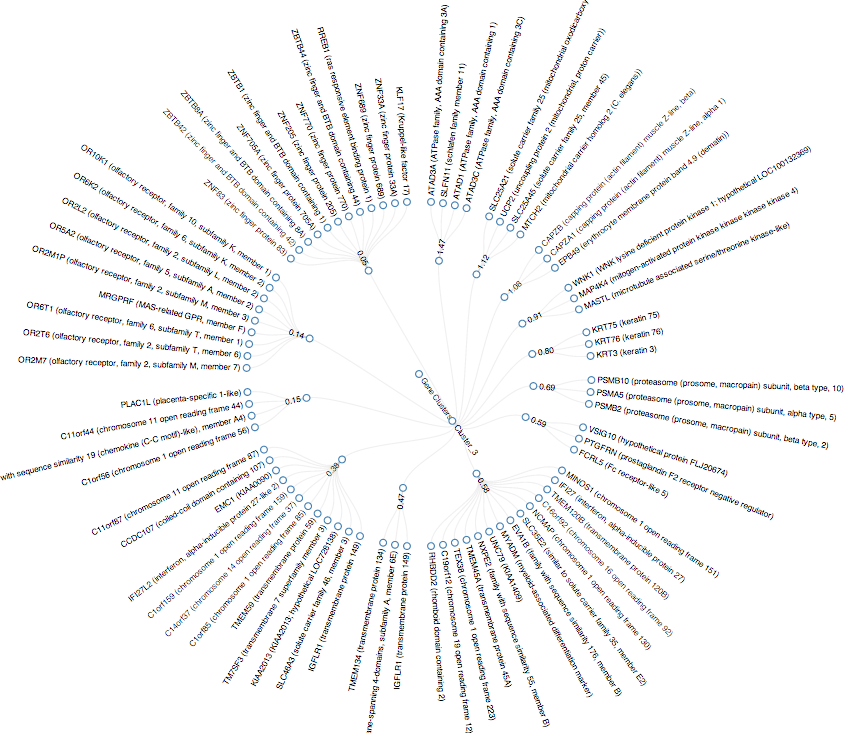
\includegraphics[height=3in]{dendrogram.png}
\caption{Dendrogram describing a cluster using our visualization tool.}
\label{fig:dendrogram}
\end{figure}



\subsection{Visualization}
In order to make expression trend analysis easier from a clinical standpoint, we created a browser-based visualization tool using \verb!d3! that provides normalized/denormalized expression trends by cluster, dendrograms for cluster annotation, and word clouds for a text summary of \verb!DAVID! gene groups by cluster.
\section{Future Goals}


We could integrate this with the SMART Genomics API to make our tool usable for all time series of gene expression.
\section{Commetary on experience}
Iris: I learned a lot on how to pull data and to compare results with the ones in a paper. I also learned a lot about

\section{Commentary on peer-review process}
Iris: I thought that it was good to get feedback, but at the same time, our proposal was missing a lot of detail on purpose because we were not sure at the time exactly on what we were going to do, and a lot of the feedback was on lack of detail, which was not that helpful. It was nice to see other people's ideas.

\section{Division of labor}

Iris: I did some of the alignment, enrichment analysis, and clustering and helped get jobs running on Broad clusters. I also did the processing for the GSE675 dataset.

\section{Acknowledgements}
Thanks to Gerald Quon, Manolis Kellis, and Maxim Wolf for their help on our project.

\begin{thebibliography} {0}

\bibitem{Snyder} Chen R, Mias G I, Li-Pook-Than J, Jiang L, et al (2012). Personal Omics profiling reveals dynamic molecular and medical phenotypes. Cell 148, 1293-1307.

\bibitem{Gerald} Gerald Quon.

\bibitem{DAVID} Huang DW, Sherman BT, Lempicki RA (2009). Systematic and integrative analysis of large gene lists using DAVID Bioinformatics Resources. Nature Protoc 4(1), 44-57.

\bibitem{webservice} Huang DW, Sherman BT, Lempicki RA (2009). Bioinformatics enrichment tools: paths toward the comprehensive functional analysis of large gene lists. Nucleic Acids Res. 37(1), 1-13.

\bibitem{GSE675} Browne EP, Wing B, Coleman D, Shenk T. Altered cellular mRNA levels in human cytomegalovirus-infected fibroblasts: viral block to the accumulation of antiviral mRNAs. J Virol 2001 Dec;75(24):12319-30. PMID: 11711622


\end{thebibliography}

\end{document}
